% ============================================================
% 31-bezier-generic-explained.tex
% Compile with:  pdflatex -shell-escape 31-bezier-generic-explained.tex
% Both PNGs must be in the same folder. Run twice for TOC.
% ============================================================

\documentclass[12pt, a4paper]{article}

\usepackage[T1]{fontenc}
\usepackage[utf8]{inputenc}
\usepackage{lmodern}
\usepackage[top=2.5cm, bottom=2.5cm, left=2.8cm, right=2.8cm]{geometry}
\usepackage{graphicx}
\usepackage{float}
\usepackage[dvipsnames]{xcolor}

\definecolor{codebg}{RGB}{248,248,248}
\definecolor{rulecolor}{RGB}{180,180,180}
\definecolor{examplebg}{RGB}{240,248,255}
\definecolor{examplerule}{RGB}{100,149,237}
\definecolor{notebg}{RGB}{255,250,230}
\definecolor{noterule}{RGB}{210,180,50}

\usepackage{minted}
\setminted[julia]{
  bgcolor=codebg, frame=leftline, framerule=1.5pt,
  rulecolor=rulecolor, linenos=false, fontsize=\small,
  breaklines=true, tabsize=4, style=friendly,
}

\usepackage{amsmath}
\usepackage{amssymb}
\usepackage{tikz}
\usetikzlibrary{shapes.geometric, arrows.meta, positioning}
\usepackage{mdframed}

\newmdenv[backgroundcolor=examplebg, linecolor=examplerule,
  linewidth=1.5pt, leftline=true, rightline=false,
  topline=false, bottomline=false,
  innerleftmargin=10pt, innerrightmargin=8pt,
  innertopmargin=6pt, innerbottommargin=6pt,
  skipabove=6pt, skipbelow=4pt]{examplebox}

\newmdenv[backgroundcolor=notebg, linecolor=noterule,
  linewidth=1.5pt, leftline=true, rightline=false,
  topline=false, bottomline=false,
  innerleftmargin=10pt, innerrightmargin=8pt,
  innertopmargin=6pt, innerbottommargin=6pt,
  skipabove=6pt, skipbelow=4pt]{notebox}

\usepackage[colorlinks=true, linkcolor=black, urlcolor=MidnightBlue]{hyperref}
\usepackage{booktabs}
\usepackage{needspace}
\usepackage{parskip}
\usepackage{titlesec}
\usepackage{fancyhdr}
\usepackage{datetime2}

\titleformat{\section}
  {\large\bfseries\color{MidnightBlue}}{\thesection.}{0.6em}{}
  [\vspace{-4pt}\rule{\linewidth}{0.4pt}]
\titleformat{\subsection}
  {\normalsize\bfseries\color{BrickRed}}{\thesubsection.}{0.5em}{}
\titleformat{\subsubsection}
  {\normalsize\bfseries}{\thesubsubsection.}{0.5em}{}

\pagestyle{fancy}
\fancyhf{}
\rhead{\textcolor{gray}{\small 31-bezier-generic-explained}}
\lhead{\textcolor{gray}{\small B\'ezier Generic --- GLMakie}}
\cfoot{\thepage}
\renewcommand{\headrulewidth}{0.3pt}

\newcommand{\cd}[1]{\texttt{#1}}

\title{%
  \vspace{1cm}
  {\LARGE\bfseries B\'ezier Curve: Generic (Any Degree, 2-D or 3-D)}\\[0.4em]
  {\large GLMakie Visualisation}\\[0.4em]
  {\large Code and Plot Explanation for Julia Beginners}\\[0.4em]
  {\normalsize\texttt{31-bezier-generic.jl}}
}
\author{E.R.\ Nurwijayadi}
\date{\DTMtoday}

\begin{document}

\maketitle
\thispagestyle{empty}

\begin{center}
\textit{Directed and curated by E.R.\ Nurwijayadi.
Code and explanations AI-generated.}
\end{center}

\begin{center}
\begin{minipage}{0.85\textwidth}
\small
This document explains \cd{31-bezier-generic.jl}.
This is the most architecturally complete script in the series:
a single program that handles \emph{any degree} and \emph{any dimension}
(2-D or 3-D) by switching on the \cd{CASE} constant.
It introduces \textbf{GLMakie} (the interactive backend),
a generic \cd{BezierCurve} struct, a generalised De Casteljau
loop, computed axis types (\cd{Axis} vs \cd{Axis3}),
and auto-fitted plot limits.
\end{minipage}
\end{center}

\vspace{1em}\hrule\vspace{1.5em}
\tableofcontents
\newpage


% =============================================================
\needspace{8\baselineskip}
\section{The Two Plots}
% =============================================================

\needspace{5\baselineskip}
\subsection{Case 1: Quadratic 2-D}

\begin{figure}[H]
  \centering
  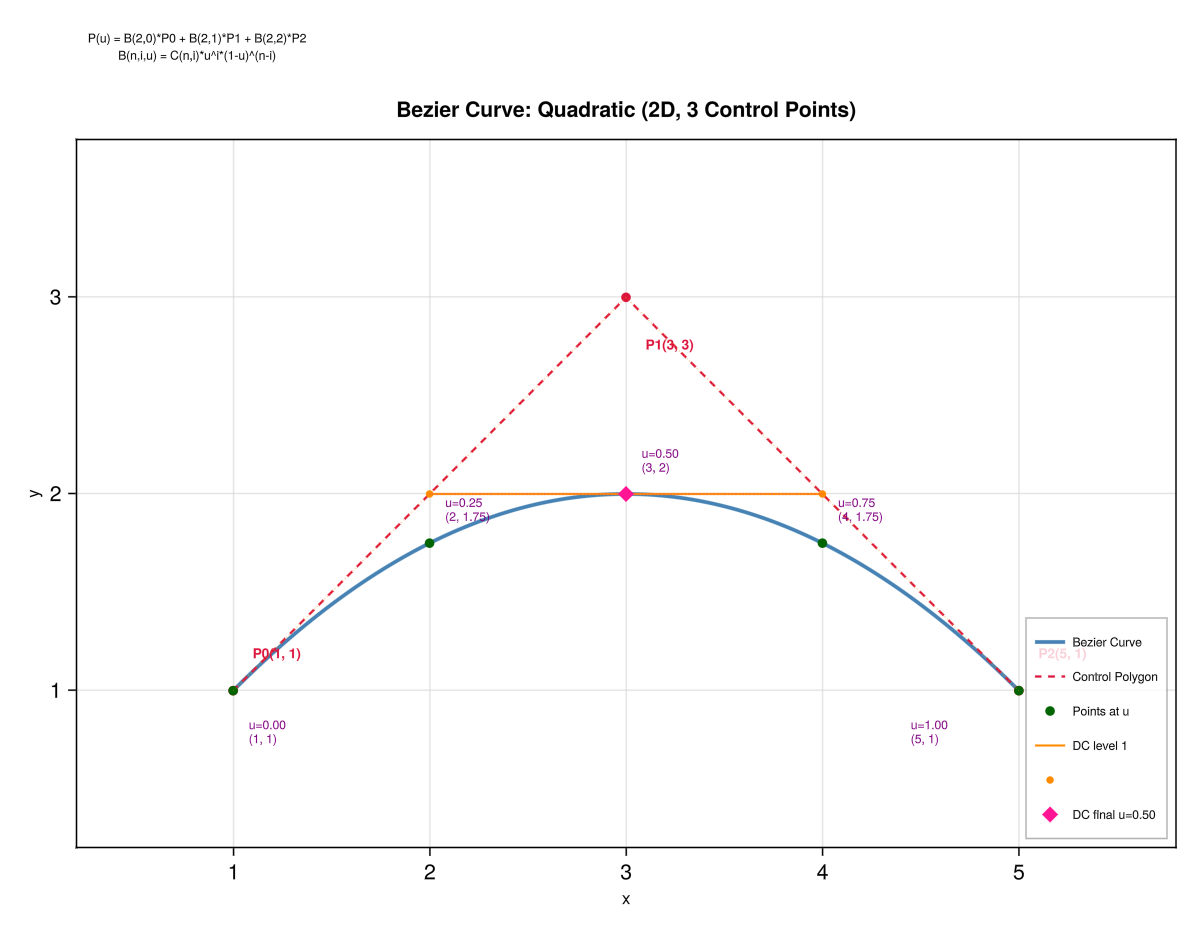
\includegraphics[width=0.92\linewidth]{31-bezier-quadratic-2d.png}
  \caption{Case~1: quadratic B\'ezier in 2-D with De Casteljau
           construction at $u=0.50$.}
\end{figure}

\needspace{5\baselineskip}
\subsection{Case 2: Quartic 3-D}

\begin{figure}[H]
  \centering
  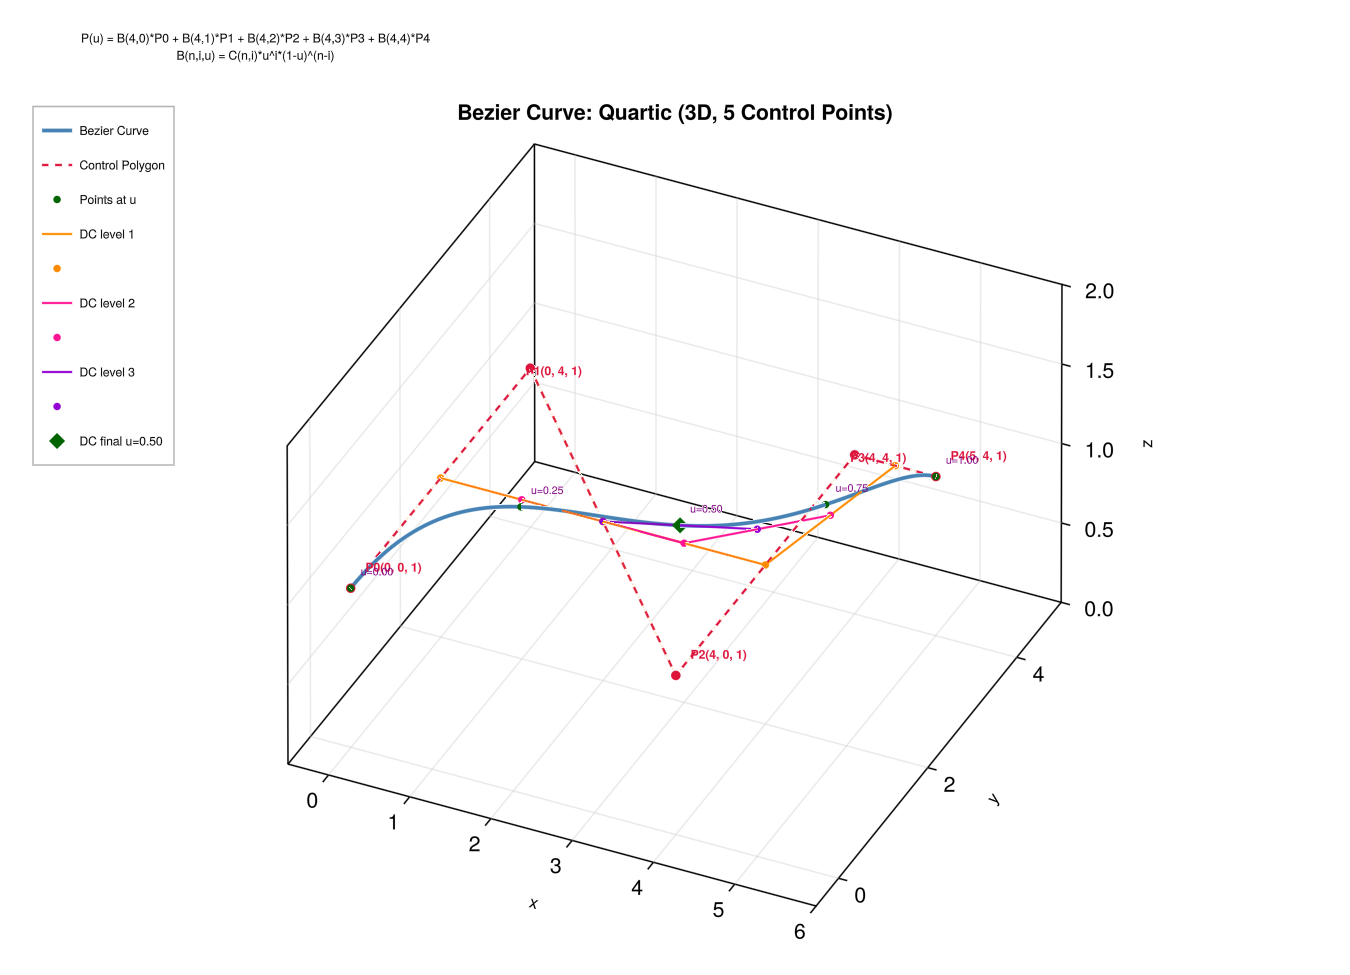
\includegraphics[width=0.92\linewidth]{31-bezier-quartic-3d.png}
  \caption{Case~2: quartic B\'ezier in 3-D with De Casteljau
           construction at $u=0.50$.
           This plot is interactive when run with GLMakie ---
           pan, zoom, and rotate with the mouse.}
\end{figure}


% =============================================================
\needspace{8\baselineskip}
\section{GLMakie: The Interactive Backend}
% =============================================================

\textit{All previous scripts used CairoMakie for static PNG output.
This script switches to GLMakie --- the interactive backend.}

\begin{center}
\begin{tabular}{lll}
\toprule
Backend & Output & Use case \\
\midrule
\cd{CairoMakie} & Static PNG, SVG, PDF & Publication figures \\
\cd{GLMakie} & Interactive window (OpenGL) & Exploration, rotation, zoom \\
\cd{WGLMakie} & Interactive browser (WebGL) & Jupyter notebooks \\
\bottomrule
\end{tabular}
\end{center}

With GLMakie, the 3-D quartic plot can be rotated with the
mouse, zoomed with the scroll wheel, and panned by dragging.
This is why the note says \textit{``the 3-D is actually can
be panned, zoom, and rotate.''} \cd{save()} still works ---
GLMakie can save a static snapshot of the current view to PNG.

Install once with:
\begin{minted}{julia}
import Pkg; Pkg.add("GLMakie")
\end{minted}


% =============================================================
\needspace{8\baselineskip}
\section{The Generic \texttt{BezierCurve} Struct}
% =============================================================

\begin{minted}{julia}
struct BezierCurve
    points ::Matrix{Float64}   # (n x dim)
    n      ::Int               # number of control points
    degree ::Int
    dim    ::Int               # 2 or 3
end

function BezierCurve(points::Matrix{Float64})
    n = size(points, 1)
    BezierCurve(points, n, n-1, size(points, 2))
end
\end{minted}

This struct replaces all the specialised structs from
previous scripts (\cd{BezierQuadratic}, \cd{BezierQuartic},
\cd{DeCasteljauQuartic}, etc.) with one generic type.

\cd{dim = size(points, 2)} reads the number of columns ---
2 for a 2-D curve, 3 for a 3-D curve.
\cd{degree = n - 1} is always one less than the number
of control points.

The constructor derives all four fields from the matrix
alone.
The caller only provides \cd{points} and the struct
figures out everything else.

\begin{examplebox}
\textbf{Case 1 (quadratic 2-D):}
\cd{points} is $3\times2$ $\Rightarrow$ \cd{n=3, degree=2, dim=2}

\textbf{Case 2 (quartic 3-D):}
\cd{points} is $5\times3$ $\Rightarrow$ \cd{n=5, degree=4, dim=3}
\end{examplebox}

\needspace{5\baselineskip}
\subsection{Helper functions}

\begin{minted}{julia}
function degree_name(bz::BezierCurve)
    names = Dict(2=>"Quadratic", 3=>"Cubic", 4=>"Quartic", 5=>"Quintic")
    get(names, bz.degree, "Degree-$(bz.degree)")
end

dim_name(bz::BezierCurve) = bz.dim == 3 ? "3D" : "2D"
\end{minted}

\cd{degree\_name} converts the degree integer to a human
name, with a fallback \cd{"Degree-N"} for unknown degrees.
\cd{dim\_name} is a one-liner returning \cd{"3D"} or \cd{"2D"}.

Both are used to build the plot title dynamically:
\begin{minted}{julia}
title = "Bezier Curve: $(degree_name(bz)) ($(dim_name(bz)), $(bz.n) Control Points)"
\end{minted}

This produces \cd{"Bezier Curve: Quadratic (2D, 3 Control Points)"}
for Case~1 and \cd{"Bezier Curve: Quartic (3D, 5 Control Points)"}
for Case~2 --- without any \cd{if/else}.


% =============================================================
\needspace{8\baselineskip}
\section{Generic Math Functions}
% =============================================================

\needspace{5\baselineskip}
\subsection{\texttt{bernstein} --- standalone basis function}

\begin{minted}{julia}
function bernstein(n::Int, i::Int, u::Float64)
    binomial(n, i) * u^i * (1 - u)^(n - i)
end
\end{minted}

A pure scalar function: given degree \cd{n}, index \cd{i},
and parameter \cd{u}, it returns the $i$-th Bernstein
basis value $\binom{n}{i} u^i (1-u)^{n-i}$.
This is factored out as a named function (rather than
inlined) because it is called inside a generator sum.

\needspace{5\baselineskip}
\subsection{\texttt{bz\_point} --- generic point via generator sum}

\begin{minted}{julia}
function bz_point(bz::BezierCurve, u::Float64)
    sum(bernstein(bz.degree, i-1, u) .* bz.points[i,:] for i in 1:bz.n)
end
\end{minted}

This computes
$P(u) = \sum_{i=0}^{n} B(n,i,u) \cdot P_i$
in a single \cd{sum(generator)} expression.

For each \cd{i} from 1 to \cd{bz.n}, it computes
\cd{bernstein(...)} (a scalar) broadcast-multiplied by
\cd{bz.points[i,:]} (a length-\cd{dim} row vector).
The \cd{sum} accumulates these vectors element-wise.

The result is a length-\cd{dim} vector of \cd{Float64}
--- either \cd{[x, y]} or \cd{[x, y, z]} depending on
the curve's dimension.
No \cd{if is\_3d} branching needed.

\begin{examplebox}
\textbf{For Case 1 (quadratic 2-D) at $u = 0.5$:}

\cd{bz.degree = 2}, \cd{bz.n = 3}

\medskip
\begin{tabular}{llll}
\toprule
$i$ & \cd{bernstein(2, i-1, 0.5)} & \cd{bz.points[i,:]} & product \\
\midrule
1 & $B(2,0,0.5) = 0.25$ & $[1,1]$ & $[0.25, 0.25]$ \\
2 & $B(2,1,0.5) = 0.50$ & $[3,3]$ & $[1.50, 1.50]$ \\
3 & $B(2,2,0.5) = 0.25$ & $[5,1]$ & $[1.25, 0.25]$ \\
\bottomrule
\end{tabular}

\medskip
Sum: $[0.25+1.50+1.25,\; 0.25+1.50+0.25] = [3.0, 2.0]$ \checkmark
\end{examplebox}

\needspace{5\baselineskip}
\subsection{\texttt{de\_casteljau} --- generalised while loop}

\begin{minted}{julia}
function de_casteljau(bz::BezierCurve, u::Float64)
    levels  = Matrix{Float64}[copy(bz.points)]
    current = copy(bz.points)
    while size(current, 1) > 1
        n = size(current, 1)
        current = vcat([(
            (1-u) .* current[j,:] .+ u .* current[j+1,:]
        )' for j in 1:n-1]...)
        push!(levels, current)
    end
    return levels
end
\end{minted}

This is the fully generalised De Casteljau algorithm.
It replaces the fixed four-step \cd{dc\_steps} from
script~22 with a \cd{while} loop that runs until
only one row remains.

\textbf{\cd{Matrix\{Float64\}[copy(bz.points)]}:}
Creates a \cd{Vector\{Matrix\{Float64\}\}} --- a vector
whose elements are matrices --- initialised with one
element: a copy of the control point matrix.
The type annotation \cd{Matrix\{Float64\}[...]} is
needed so Julia knows what type of vector to create.

\textbf{\cd{copy(bz.points)}:}
Makes an independent copy of the matrix.
Without \cd{copy}, modifying \cd{current} would also
modify \cd{bz.points} because they would share the same
memory.

\textbf{The \cd{while} loop:}
Each iteration applies one reduction step --- identical
to \cd{reduce\_level} from script~22 but written inline
here.
\cd{push!(levels, current)} appends the new level matrix
to the growing vector.

\textbf{Return value:}
\cd{levels} is a \cd{Vector\{Matrix\{Float64\}\}} with
\cd{degree + 1} elements:
\cd{levels[1]} is L0 ($n$ rows),
\cd{levels[2]} is L1 ($n-1$ rows), \ldots,
\cd{levels[end]} is the final level (1 row).

\begin{examplebox}
\textbf{For Case 1 (quadratic) at $u=0.5$:}

Initial \cd{current}: $3\times2$ matrix (L0).

\textbf{Iteration 1:} \cd{size(current,1) = 3 > 1}.
Reduces to $2\times2$ (L1). \cd{push!} appends to \cd{levels}.

\textbf{Iteration 2:} \cd{size(current,1) = 2 > 1}.
Reduces to $1\times2$ (L2 = final). \cd{push!} appends.

\textbf{Iteration 3:} \cd{size(current,1) = 1}. Loop exits.

\cd{levels} has 3 elements: L0, L1, L2.
\cd{levels[end] = [[3.0, 2.0]]} (the curve point). \checkmark

\medskip
\textbf{For Case 2 (quartic) at $u=0.5$, the loop runs 4 times}
producing \cd{levels} with 5 elements: L0 through L4.
\end{examplebox}


% =============================================================
\needspace{8\baselineskip}
\section{\texttt{draw\_and\_save} --- Branching on Dimension}
% =============================================================

\textit{This is the most branching-heavy function in the series.
The \cd{is\_3d} flag controls whether to use \cd{Axis3} or
\cd{Axis}, whether to pass two or three coordinate arguments
to drawing functions, and how to compute label offsets.}

\needspace{5\baselineskip}
\subsection{Conditional axis creation}

\begin{minted}{julia}
is_3d = bz.dim == 3
title = "Bezier Curve: $(degree_name(bz)) ..."

fig = Figure(size = (is_3d ? 900 : 800, is_3d ? 650 : 620), ...)

if is_3d
    ax = Axis3(fig[1,1], title=title, ..., elevation=..., azimuth=...)
else
    ax = Axis(fig[1,1], title=title, ...)
end
\end{minted}

\cd{is\_3d} is a plain \cd{Bool} variable computed once
and reused throughout.

\textbf{Ternary size:}
\cd{is\_3d ? 900 : 800} is Julia's ternary operator
--- evaluates to 900 if \cd{is\_3d} is true, 800 otherwise.
The figure is slightly wider and taller for 3-D to give
the \cd{Axis3} room for its depth cues.

Both branches create a variable called \cd{ax}.
Julia's type system allows \cd{ax} to be either an
\cd{Axis} or an \cd{Axis3} --- both are subtypes of
\cd{AbstractAxis} and both accept the same drawing
functions (\cd{lines!}, \cd{scatter!}, \cd{text!}).

\needspace{5\baselineskip}
\subsection{Dynamic control point labels}

\begin{minted}{julia}
for i in 1:bz.n
    pt     = cp[i,:]
    coords = join([@sprintf("%.4g", v) for v in pt], ", ")
    name   = "P$(i-1)($coords)"
    dy     = i % 2 == 1 ? 0.15 : -0.28
    ...
end
\end{minted}

\textbf{The \cd{join} + \cd{@sprintf} pattern:}
The list comprehension \cd{[@sprintf("\%.4g", v) for v in pt]}
formats each coordinate with \cd{"\%.4g"} (up to 4
significant figures, dropping trailing zeros).
\cd{join(..., ", ")} concatenates the results with
commas.
For \cd{pt = [0.0, 4.0, 1.0]}, this produces
\cd{"0, 4, 1"}.
This works for both 2-D and 3-D without any branching
--- the comprehension adapts to however many coordinates
the point has.

\textbf{\cd{dy = i \% 2 == 1 ? 0.15 : -0.28}:}
Alternates the vertical offset between positive
(above the point) and negative (below) based on
whether the index is odd or even.
This staggers consecutive labels so they don't
overlap, without needing a hand-crafted offset array.

\begin{examplebox}
\textbf{Labels generated for Case 1:}

\medskip
\begin{tabular}{llll}
\toprule
$i$ & \cd{pt} & \cd{coords} & \cd{name} \\
\midrule
1 & \cd{[1,1]} & \cd{"1, 1"} & \cd{"P0(1, 1)"} \\
2 & \cd{[3,3]} & \cd{"3, 3"} & \cd{"P1(3, 3)"} \\
3 & \cd{[5,1]} & \cd{"5, 1"} & \cd{"P2(5, 1)"} \\
\bottomrule
\end{tabular}

\cd{dy} alternates: $i=1$ (odd) $\to$ \cd{0.15};
$i=2$ (even) $\to$ \cd{-0.28};
$i=3$ (odd) $\to$ \cd{0.15}.
\end{examplebox}

\needspace{5\baselineskip}
\subsection{Highlighted point labels: computed offsets}

\begin{minted}{julia}
for (i, u) in enumerate(u_highlight)
    pt     = hpts[i,:]
    coords = join([@sprintf("%.3g", v) for v in pt], ", ")
    lbl    = @sprintf("u=%.2f\n(%s)", u, coords)
    dx     = u == 1.0 ? -0.55 : 0.08
    dy     = u in (0.0, 1.0) ? -0.28 : 0.10
    text!(ax, pt[1]+dx, pt[2]+dy, ...)
end
\end{minted}

The 2-D label offsets are computed from the $u$ value
using two conditions:

\cd{dx}: \cd{-0.55} at $u=1$ (shift left so the label
doesn't run off the right edge), \cd{0.08} everywhere else.

\cd{dy}: \cd{-0.28} at $u=0$ and $u=1$ (shift below,
where there is space), \cd{0.10} everywhere else
(shift above).

\cd{u in (0.0, 1.0)} uses Julia's \cd{in} operator to
check membership in a tuple --- a compact alternative
to \cd{u == 0.0 || u == 1.0}.

\needspace{5\baselineskip}
\subsection{The De Casteljau drawing loop}

\begin{minted}{julia}
levels = de_casteljau(bz, u_dc)
for lv in 2:length(levels)
    pts      = levels[lv]
    col      = COLOR_DC[min(lv-1, length(COLOR_DC))]
    is_final = (lv == length(levels))
    lbl      = is_final ? @sprintf("DC final u=%.2f", u_dc)
                        : "DC level $(lv-1)"

    if !is_final
        lines!(ax, pts[:,1], pts[:,2], [pts[:,3] if is_3d]..., ...)
    end
    scatter!(ax, ...,
        marker = is_final ? :diamond : :circle,
        label  = is_final ? lbl : "")

    # Vertical connectors (interpolation triangle edges)
    prev = levels[lv-1]
    for j in 1:size(pts,1)
        for k in [j, j+1]
            seg_x = [prev[k,1], pts[j,1]]
            seg_y = [prev[k,2], pts[j,2]]
            lines!(ax, seg_x, seg_y, ...,
                color=(col, 0.35), linewidth=0.8, linestyle=:dot)
        end
    end
end
\end{minted}

\textbf{\cd{COLOR\_DC[min(lv-1, length(COLOR\_DC))]}:}
\cd{COLOR\_DC = [:darkorange, :deeppink, :darkviolet, :darkgreen]}.
Index \cd{lv-1} starts at 1 (for L1) and goes up to
\cd{degree} (for the final level).
\cd{min(lv-1, length(COLOR\_DC))} clamps the index to
the length of \cd{COLOR\_DC}, preventing an out-of-bounds
error for curves of degree higher than 4.
For a quartic, \cd{lv-1} goes 1, 2, 3, 4 --- exactly
the four colours available.

\textbf{\cd{label = is\_final ? lbl : ""}:}
Only the final level point (the diamond) gets a legend
entry.
All intermediate level lines and dots use \cd{label = ""}
to suppress their legend entries.

\textbf{Vertical connectors:}
For each point \cd{pts[j]} in the current level,
two dotted lines are drawn: one from \cd{prev[j]}
to \cd{pts[j]}, and one from \cd{prev[j+1]} to
\cd{pts[j]}.
These are the two edges of the interpolation triangle
for that point --- visually showing \emph{which two
parent points} each child point was interpolated from.
The \cd{(col, 0.35)} alpha makes them semi-transparent
so they don't dominate the plot.

\begin{examplebox}
\textbf{Connector drawing for Case 1 (quadratic), L1 at $u=0.5$:}

L0 (\cd{prev}) has 3 rows: $P_0, P_1, P_2$.
L1 (\cd{pts}) has 2 rows: $Q_0, Q_1$.

For $j=1$ ($Q_0$): draws \cd{prev[1]} $\to$ \cd{pts[1]}
and \cd{prev[2]} $\to$ \cd{pts[1]}.
That is, two dotted lines converging at $Q_0$ from
$P_0$ and $P_1$.

For $j=2$ ($Q_1$): draws \cd{prev[2]} $\to$ \cd{pts[2]}
and \cd{prev[3]} $\to$ \cd{pts[2]}.
Two dotted lines converging at $Q_1$ from $P_1$ and $P_2$.

This creates the ``V'' shapes visible on the quadratic plot
showing the interpolation ancestry of each level point.
\end{examplebox}

\needspace{5\baselineskip}
\subsection{Dynamic equation text}

\begin{minted}{julia}
n     = bz.degree
terms = join(["B($n,$(i-1))*P$(i-1)" for i in 1:bz.n], " + ")
eq    = "P(u) = $terms\nB(n,i,u) = C(n,i)*u^i*(1-u)^(n-i)"
Label(fig[0, 1], eq, fontsize=8, font="Courier New", ...)
\end{minted}

The equation string is built dynamically from the degree
and number of control points.

For Case~1 (quadratic, 3 points):
\cd{"P(u) = B(2,0)*P0 + B(2,1)*P1 + B(2,2)*P2"}

For Case~2 (quartic, 5 points):
\cd{"P(u) = B(4,0)*P0 + ... + B(4,4)*P4"}

No hardcoded strings --- the equation adapts to any
degree automatically.

\needspace{5\baselineskip}
\subsection{Auto-fitted 2-D limits}

\begin{minted}{julia}
if !is_3d
    all_x = vcat(cp[:,1], cpts[:,1])
    all_y = vcat(cp[:,2], cpts[:,2])
    m = 0.8
    xlims!(ax, minimum(all_x)-m, maximum(all_x)+m)
    ylims!(ax, minimum(all_y)-m, maximum(all_y)+m)
end
\end{minted}

For the 2-D case, instead of hardcoding
\cd{limits = (0.5, 6.0, 0.5, 3.5)},
the limits are computed from the actual data.

\cd{vcat(cp[:,1], cpts[:,1])} concatenates the $x$
coordinates of the control points and the 300 curve
points into one vector.
\cd{minimum} and \cd{maximum} find the extremes.
Adding/subtracting margin \cd{m = 0.8} gives padding.

\textbf{\cd{xlims!(ax, xmin, xmax)} and \cd{ylims!(ax, ymin, ymax)}:}
These Makie functions set the axis limits after the
axis has already been created.
They are the post-hoc equivalent of passing
\cd{limits = (...)} to \cd{Axis(...)}.

This approach is necessary here because the limits
depend on the data, which is only available after
\cd{bz\_curve} has been called.

\begin{examplebox}
\textbf{Auto-fitted limits for Case 1:}

Control point $x$: min $= 1$, max $= 5$.

Curve $x$: min $\approx 1$, max $\approx 5$.

Combined: min $= 1$, max $= 5$.

With margin 0.8: \cd{xlims!(ax, 0.2, 5.8)}.

Similarly $y$: control range $[1, 3]$, curve range $[1, 2]$,
combined $[1, 3]$, with margin: \cd{ylims!(ax, 0.2, 3.8)}.
\end{examplebox}


% =============================================================
\needspace{8\baselineskip}
\section{Type Map}
% =============================================================

\tikzset{
  structbox/.style={rectangle, rounded corners=4pt,
    draw=MidnightBlue, line width=1.5pt, fill=examplebg,
    text width=3.6cm, align=center, font=\small\bfseries, inner sep=8pt},
  funcbox/.style={rectangle, rounded corners=2pt,
    draw=gray!60, line width=1pt, fill=white,
    text width=3.6cm, align=center, font=\small, inner sep=7pt},
  entrybox/.style={rectangle, rounded corners=4pt,
    draw=BrickRed, line width=1.5pt, fill=notebg,
    text width=2.4cm, align=center, font=\small\bfseries, inner sep=8pt},
  myarrow/.style={-Stealth, thick, draw=gray!70},
  bluearrow/.style={-Stealth, thick, draw=MidnightBlue},
  redarrow/.style={-Stealth, thick, draw=BrickRed!80},
  arrowlabel/.style={font=\footnotesize\itshape, fill=white, inner sep=2pt}
}

\begin{center}
\begin{tikzpicture}[node distance=1.5cm and 2.8cm]

  \node[structbox] (bz) {%
    \texttt{BezierCurve}\\[3pt]
    \footnotesize\normalfont
    \texttt{points, n, degree, dim}\\
    \textit{any degree, any dim}
  };

  \node[funcbox, below left=1.5cm and 0.2cm of bz] (math) {%
    \textbf{Math functions}\\[2pt]
    \footnotesize\normalfont
    \texttt{bernstein(n,i,u)}\\
    \texttt{bz\_point(bz,u)}\\
    \texttt{bz\_curve / bz\_highlight}\\
    \texttt{de\_casteljau(bz,u)}
  };

  \node[funcbox, below right=1.5cm and 0.2cm of bz] (draw) {%
    \texttt{draw\_and\_save}\\[2pt]
    \footnotesize\normalfont
    \texttt{is\_3d} branch:\\
    \texttt{Axis3} or \texttt{Axis}\\
    \textit{dynamic labels}\\
    \textit{DC while loop}\\
    \texttt{xlims!/ylims!}
  };

  \node[entrybox, right=2.2cm of bz] (main) {%
    \texttt{main()}\\[2pt]
    \footnotesize\normalfont\normalcolor
    \textit{entry point}
  };

  \draw[bluearrow] (bz)   -- node[arrowlabel,above left]{passed to} (math);
  \draw[bluearrow] (bz)   -- node[arrowlabel,above right]{passed to} (draw);
  \draw[myarrow]   (draw) -- node[arrowlabel,below]{calls} (math);
  \draw[redarrow]  (main) -- node[arrowlabel,above]{creates} (bz);
  \draw[redarrow]  (main) |- node[arrowlabel,right,pos=0.8]{calls} (draw);

\end{tikzpicture}
\end{center}


% =============================================================
\needspace{8\baselineskip}
\section{Entry Point}
% =============================================================

\begin{minted}{julia}
function main()
    data = CASE_DATA[CASE]
    bz   = BezierCurve(data.points)
    draw_and_save(bz, data.u_highlight, data.u_dc, data.output)
end

main()
\end{minted}

\cd{BezierCurve(data.points)} is the only constructor call.
Everything else --- degree, dimension, axis type, label
format, limit computation --- flows from the struct's
fields automatically.

\begin{notebox}
\textbf{How to run:}
\begin{minted}{julia}
julia 31-bezier-generic.jl
\end{minted}
Change \cd{const CASE = 1} or \cd{= 2} at the top
to switch between 2-D and 3-D.
With GLMakie, the 3-D window is interactive:
rotate with left-click drag, zoom with scroll,
pan with right-click drag.
Press Enter in the terminal to close.
\end{notebox}

\vspace{2em}\hrule\vspace{0.5em}
{\small\textcolor{gray}{%
Explanation for \texttt{31-bezier-generic.jl}
\textbar{} Directed and curated by E.R.\ Nurwijayadi
\textbar{} Code and explanations AI-generated}}

\end{document}
